% Template for PLoS
% Version 1.0 January 2009
%
% To compile to pdf, run:
% latex plos.template
% bibtex plos.template
% latex plos.template
% latex plos.template
% dvipdf plos.template

\documentclass[10pt]{article}

% amsmath package, useful for mathematical formulas
\usepackage{amsmath}
% amssymb package, useful for mathematical symbols
\usepackage{amssymb}

% graphicx package, useful for including eps and pdf graphics
% include graphics with the command \includegraphics
\usepackage{graphicx}

% cite package, to clean up citations in the main text. Do not remove.
\usepackage{cite}

% required by the coloured \Fixme and \Change macros
\usepackage{color}

% Use doublespacing - comment out for single spacing
%\usepackage{setspace}
%\doublespacing

\definecolor{ChangeColor}{rgb}{0.24,0.56,0.18}
%\definecolor{ChangeColor}{rgb}{0,0,0}
\newcommand{\Change}[1]{{\color{ChangeColor}{#1}}}

\definecolor{FixmeColor}{rgb}{1,0,0}
%\definecolor{FixmeColor}{rgb}{0,0,0}
\newcommand{\Fixme}[1]{{\color{FixmeColor}{#1}}}


% Text layout
\topmargin 0.0cm
\oddsidemargin 0.5cm
\evensidemargin 0.5cm
\textwidth 16cm
\textheight 21cm

% Bold the 'Figure #' in the caption and separate it with a period
% Captions will be left justified
\usepackage[labelfont=bf,labelsep=period,justification=raggedright]{caption}

% Use the PLoS provided bibtex style
\bibliographystyle{plos2009}

% Remove brackets from numbering in List of References
\makeatletter
\renewcommand{\@biblabel}[1]{\quad#1.}
\makeatother


% Leave date blank
\date{}

\pagestyle{myheadings}
%% ** EDIT HERE **
\newcommand{\COMMENT}[1]{{\color{red} #1 }}
\newcommand{\COM}[1]{{\color{blue} #1 }}

\graphicspath { {./figures/fig1/} {./figures/fig2/} {./figures/fig9/} {./figures/fig5/}}
\usepackage[normalem]{ulem}
\usepackage{amssymb}
\usepackage[colorlinks]{hyperref}
\usepackage{booktabs}
\usepackage{amsmath}
%\usepackage{multirow}% http://ctan.org/pkg/multirow
%\usepackage{tablefootnote}
%\usepackage{import}
\usepackage{subcaption}
\usepackage{caption}
%\usepackage[format=hang,font=small,labelfont=bf]{caption}


%% ** EDIT HERE **
%% PLEASE INCLUDE ALL MACROS BELOW

%% END MACROS SECTION

\begin{document}

% Title must be 150 characters or less
\begin{flushleft}
{\Large
\textbf{A quantitative assessment of the Hadoop framework for analyzing massively parallel DNA sequencing data}
}
% Insert Author names, affiliations and corresponding author email.
\\
Alexey Siretskiy$^{1 \ast}$,
Luca Pireddu$^{2}$,
Ola Spjuth$^{3,4}$
\\
{\bf 1} Department of Information Technology, Uppsala University, Uppsala, Sweden
 \\
{\bf 2} CRS4, Polaris, Pula, Italy
 \\
{\bf 3} Department of Pharmaceutical Biosciences, Uppsala University, Uppsala, Sweden
 \\
{\bf 4} Science for Life Laboratory, Uppsala University, Uppsala, Sweden
\\
$\ast$ E-mail: alexey.siretskiy@it.uu.se
\end{flushleft}

% Please keep the abstract between 250 and 300 words
\section*{Abstract}
New high-throughput technologies such as massively parallel sequencing have transformed the life sciences into a data-intensive field. With increasing data volumes comes the necessity to analyze data in parallel using high-performance computing resources, but doing this effectively can be laborious and challenging.
Hadoop, which has emerged over the last decade, is a framework that automatically distributes data and computation and has been shown to scale to thousands of nodes. Herein we introduce metrics and report a quantitative comparison of Hadoop to regular high-performance computing resources for aligning short reads and calling variants for five datasets of different sizes up to 250\,gigabases. In order to increase performance of existing software and obtain a better comparison we modified and wrote new analysis scripts. From the observed scaling relations we are able to draw conclusions about the perspectives of the approaches, leading to the conclusion that as data set sizes reach 100\,gigabases, the Hadoop-based pipelines become performance-competitive with a canonical high-performance cluster solution. As data sets in biological sequencing are sure to increase with time, Hadoop and similar frameworks are very interesting technologies that we envision will play a key role in the future of biological data analysis.

% Please keep the Author Summary between 150 and 200 words
% Use first person. PLoS ONE authors please skip this step.
% Author Summary not valid for PLoS ONE submissions.
\section*{Author Summary}
New experimental technologies in biology generate vast amounts of data that require
high-performance computing to analyze and store. With the increase in dataset volumes there is a need for new computational tools and technologies that can cope with the scale of data. In this paper we provide a detailed study comparing the performance of the Hadoop framework with traditional high-performance computing for data in biological sequencing. While there is an overhead in using Hadoop, we show that as sequencing data sets reach sizes of 100 gigabases Hadoop becomes an attractive option compared with traditional methods. We also show that Hadoop scales linearly while traditional systems become network-saturated at larger data sizes. As sequencing data are bound to increase in the future, Hadoop is a very interesting framework on which to base future analysis.




%%%%%%%%%%%%
% Introduction
%%%%%%%%%%%

\section*{Introduction}
%The problem: dealing with BIG data
Since its inception, massively parallel DNA sequencing, also referred to as Next Generation Sequencing~(NGS) technology, has been an extremely bountiful source of data providing insight into the workings of biological machinery~\cite{metzker, Marx:2013fk}. Decreasing sequencing costs facilitates and promotes larger and larger studies with increasingly larger data sizes. Extracting useful information from these voluminous amounts of data is transforming biology into a data-intensive discipline requiring a high-performance computing (HPC) infrastructure to produce results.  As an example of the scale of the demands, consider that a single Illumina high-throughput sequencing run produces approximately 1800\,gigabases (Gbases) corresponding to 2\,terabytes (TB) of raw data in 3 days~\cite{illumina}.

%Current practices: HPC systems
A common step of NGS data analysis consists of aligning short reads to a reference sequence and then finding the genetic variations specific to the sample.
Many of the most widespread tools for this purpose -- like BWA~\cite{bwa}, Bowtie~\cite{Langmead:2009uq} and Samtools~\cite{samtools} -- are not designed with distributed computing in mind. Many others do not even have the native ability to use multiple cores.

%Current practices: How to parallelize
The most common approach to accelerate NGS tools is to parallelize within a compute node (multi-core parallelization) using shared memory parallelism~(OMP)~\cite{openmp}, but this approach is naturally limited by the number of cores per node, which does not usually exceed~16~\cite{top500}. For the tools which do not support OMP natively -- e.g. Samtools -- variant calling can be parallelized by creating a separate process for each chromosome or using the GNU Parallel Linux utility~\cite{Tange2011a}.
It is important to note that a multi-core approach does not improve the performance of operations that are limited by local disk or network throughputs, whereas splitting the dataset and using multi-node parallelization is not generally bound by those constraints. A common way to implement multi-node parallelization is by using Message Passing Interface~(MPI)~\cite{mpi1}. However, writing efficient MPI-programs for hundreds of cores is a non-trivial task since thread synchronization (or load balancing) has to be woven into the software code, and there are only a few existing solutions available for processing sequencing data~\cite{pmap, erne, gnumap}.

Another common way to introduce parallelization into NGS analysis pipelines in Linux systems is to use custom scripting in a language such as Bash, Perl, or Python. This involves using existing utilities and cluster tools to split the data into chunks, process them on the separate nodes, and merge the results afterwards. This kind of solution benefits from both MPI-like and OMP parallelization and provides good performance, but the development requires substantial expertise in order to be efficient. Since the process is tightly coupled to the local computational cluster and network architectures, it might also be nearly impossible to re-use such developments in other settings.

%Introduce Hadoop, MR, and HDFS
%Properties of Hadoop and HDFS- data localization and programming model etc
The Map-Reduce~(MR) programming paradigm~\cite{dean.2004.mapreduce} offers a compelling alternative for running tasks in a {\it massively} parallel way. This paradigm, however, shifts the focus from the best performance to scalability, suited for managing huge datasets of sizes up to several terabytes~\cite{lin2010}.
The most prevalent open source implementation of Map-Reduce is Hadoop~\cite{hadoop,Hadoop:Guide}.
The Hadoop~MR framework provides automatic distribution of computations over many nodes as well as automatic failure recovery (failure of individual jobs or computing nodes by storing multiple copies of data on different nodes), and automated collection of results~\cite{Hadoop:Guide}. Hadoop Distributed File System~(HDFS) is a complementary component that stores data by automatically distributing it over the entire cluster, writing data blocks onto the local disk of each node and therefore effectively enabling moving the computation to the data and thus reducing network traffic. HDFS provides a storage system where the bandwidth and size scales with the number of nodes in the cluster~\cite{Sammer:2012}, which is very different from the properties of the usual HPC cluster network architecture.

%Manuscript focus: When is Hadoop currently an appealing alternative
%Introduce what we did in the manuscript.
In this manuscript we focus on the question of {\it when} is Hadoop an appealing alternative to the programs for DNA-seq analysis generally found in~HPC centers.
Since the Hadoop framework poses a significant performance overhead, we seek to estimate the average data size at which point it starts to pay off from a performance perspective. We also study the analysis execution times for datasets of different sizes and evaluate Hadoop and the HPC approaches from a scaling perspective.


%%%%%%%%%%%
% Methods
%%%%%%%%%%%
% You may title this section "Methods" or "Models". 
% "Models" is not a valid title for PLoS ONE authors. However, PLoS ONE
% authors may use "Analysis" 
\section*{Methods}


\subsection*{Analysis pipelines}

For our work to determine when Hadoop is an appealing option for genomic
sequence analysis, we chose as a representative 
use case for our experiments the task of identifying
single-nucleotide polymorphisms (SNPs) from short-read data.  We constructed
two pipelines that perform the same task: one that runs in an HPC environment
and the other on the Hadoop platform.  Although there are many different
approaches and software tools to perform this task in an HPC environment~\cite{Li:2013fk} there is only a limited
number of options for Hadoop. Given this limitation, we decided to keep the
analysis pipeline as simple as possible to ensure a fair comparison between the
two platforms.
%(e.g., GATK~\cite{gatk}, \Fixme{Other example? Otherwise none}), 

\begin{enumerate}
\item HPC approach
\subitem Short-read alignment: Bowtie~ver.~0.12.8
\subitem SNP calling: Samtools~ver.~0.1.19
\item Hadoop approach: Crossbow
\subitem Short-read alignment: Bowtie~ver.~0.12.8
\subitem SNP calling: SOAPsnp~1.02
\end{enumerate}


In the HPC pipeline, reads were aligned with Bowtie~\cite{Langmead:2009uq}, followed by sorting the aligned reads and~SNP calling with Samtools~\cite{samtools}. The Bowtie aligner natively implements~OMP -- therefore, using 8 cores on the same computer will theoretically produce a result 8 times faster than using a single core. Likewise, Samtools (as of version~0.1.19) also offers shared memory parallelism for several of its functions. Where available these features were used to improve the analysis speed. The exact workflow used is available from Github~\cite{code_repo_bash}.


The equivalent Hadoop-based pipeline was implemented with Crossbow~\cite{Langmead:2009kx}. The input
data and the indexed genome reference were copied to Hadoop's storage
system~(HDFS) before starting the experiments.  Specifically, the storage volume
containing the input data was mounted with SSHFS to one of the Hadoop nodes,
from where the \texttt{bzip2}-compressed data were transferred to the HDFS.
Crossbow implements a short pipeline that pre-processes the input data, transforming it into a format suitable for the alignment stage, and then continues to use Bowtie for alignment and SoapSNP~\cite{soapsnp} to call SNPs.  Unfortunately, unlike Crossbow's main program, its preprocessor does not scale well to large datasets (it is not implemented as a MR program). Due to this limitation, this basic step threatened to be the most time-consuming procedure in our test pipeline and bias our experiments. To overcome this bottleneck we substituted Crossbow's preprocessor with our own MR implementation (available from Github~\cite{code_repo_mr}). Our implementation is described in Section~{\it MapReduce-based Data Preprocessor}.


\subsection*{Datasets}
For our experiments we used three publicly available DNA-seq datasets~(I--III),
a synthetic dataset~(IV) of {\it A.thaliana} -- the well-known model plant --
and a dataset (V) of two {\it H.sapiens} individuals
(Table~\ref{table:datasets}). Datasets I-III and V are composed of Illumina
HiSeq sequencing data. Additional information about the source of the datasets is
provided in the Supplementary Material section.

All data was standardized to FASTQ format and compressed. The
\texttt{bzip2} compression codec was selected as it provides very good compression
and is splittable by Hadoop, meaning that the archive can be expanded in a
parallel manner allowing Hadoop to process multiple segments simultaneously.
Also, due to the lack of a standard FASTQ record id, which is
required by our test pipelines to extract the read number, we also standardized
the read ids in the datasets by generating new ids based on the SHA-1 hash
function and labelled read mates with ``.1" and ``.2" suffixes.

\subsection*{MapReduce-based Data Preprocessor}
\label{sec:preprocessor}


The Crossbow package includes a native preprocessing stage that provides great
flexibility in delivering the data to the Hadoop cluster; it can autonomously
download data from Amazon S3, FTP and HTTP servers over the
Internet~\cite{Langmead:2009kx}. However, this preprocessor does not parallelize
its operations. In theory one can manually introduce some degree of
parallelization by manually splitting the original input read data into smaller
files and to explicitly configuring Crossbow's preprocessor to download each one
(this is done by listing all of them in a special \textit{manifest file}).

%\footnote{the same holds for Myrna, a cloud-based solution for differential expression analysis}
We reimplemented the main functionality in the Crossbow preprocessor as an MR
program to benefit from its massively parallel nature. The new MR preprocessor
was implemented in Python using the Hadoop streaming library.
%\Fixme{Consider deleting the following implementation detail.}
%To route both reads of the same pair to the same Reducer, a secondary key-sorting mechanism was employed.
The resulting program efficiently processes short reads produced by different
versions of the Illumina sequencing platform as well as FASTQ files generated
from SRA files (NCBI Sequence Read Archive~\cite{ncbi-sra}). However, the
Hadoop-based approach imposes the requirement that the input data is stored
where the Hadoop nodes can access it, which is in our opinion does not bias the comparison since
sequencing platforms in the general case have direct access to storage and
computing facilities.


\subsection*{Computational resources}
To run the HPC analysis pipeline we used a computational cluster at UPPMAX,
which is heavily used for analysis of NGS-data~\cite{lampa}.
Data and reference genomes were stored on a parallel, shared storage system.
On the other hand, the Hadoop test platform was deployed on a private cloud at
UPPMAX using the OpenNebula~\cite{opennebula} cloud manager. The cluster was
configured with Cloudera Hadoop distribution version~2.0.0-mr1-cdh4.5.0~\cite{cloudera}.
For the fully detailed hardware configuration of the two computational resources
please see the Supplementary Material section.



%%%%%%%%%%%%
% Results
%%%%%%%%%%%%
% Results and Discussion can be combined.
\section*{Results}

%As described in the Methods Section, we constructed two pipelines for identifying single-nucleotide polymorphisms
%(SNPs) from short-read data, one based on Hadoop and the other on regular HPC
%with a batch processing system (hereafter referred to as the HPC method)
%(Methods).  

We executed the two pipelines for each of the five 
datasets on the HPC and Hadoop platforms, and measured the wall-clock run time for each pipeline stage.  
All experiments were repeated at least three times, 
and the results averaged to obtain a data point for the
particular combination of data size and computational platform.

\subsection*{Accuracy of Pipelines}
Since our HPC and Hadoop pipelines use different~SNP callers (Samtools and
SOAPsnp) we could not expect them to deliver perfectly
matching SNP lists. Instead, we verified the accuracy of the test pipelines by
verifying their ability to correctly identify the mutation $C\rightarrow T$ on
chromosome 4 at position $16702262$~\cite{schneeberger} in Dataset I.



\subsection*{Performance evaluation of MR-based preprocessing stage}

To quantify the processing time saved by adopting the MR approach for
preprocessing the read data, we ran an
experiment comparing the new preprocessor described in
Section~{\it MapReduce-based Data Preprocessor} to the original preprocessor furnished with
Crossbow.  To further validate our strategy, we also compared the performance of
our MapReduce approach to a different parallelization strategy based on a custom Bash script
that uses all processing cores available on a single computing node to accelerate the operation (see
Supplementary Material for details of the implementation). This program read its
input directly from conventional HPC storage, rather than HDFS\@.  The experiment
was run on Datasets II, III, and IV\@.  The Hadoop cluster used was configured
with 56 cores (7 slave nodes) while the Bash approach ran on a single node
equipped with 16 CPU cores.


%\footnote{other options like splittable LZO are also possible}

Table~\ref{table:preprocess} shows the results of the experiment, and we see that all 
of of the parallel approaches are much faster than the original tool, for
all dataset sizes.  Also, we noticed that the difference between the Bash and Hadoop
approaches is minimal when running on Dataset II\@.  Indeed, with the relatively
small dataset size the overhead incurred by the Hadoop framework likely
overwhelms the useful compute time used for each available CPU core. However,
with increasing input size the superior scalability of MR becomes apparent, with
the largest dataset requiring less than half the time of the Bash
approach to be processed. At the same time, it is important to also notice that
the Hadoop approach employed approx.\ 1.6 times more CPU time compared to the
Bash approach.

%ran on a single HPC node, utilizes multiple cores, with the limiting factor
%being \sout{the hard disk IO performance.}\COM{More correctly to say, that the
%pipe is not filled completely. i.e. the degree of achieved parallelization does
%not utilize all 16 cores. Perhaps not the best bash commands etc.} , which
%effectively leaves with 5-7 cores of 16. \COMMENT{awkward}

\subsection*{Scalability of HPC and Hadoop approaches}
Given the wide range in genome dataset sizes processed in practice -- e.g.
exomes and whole-genome sequencing at various depths -- it is
important to understand the scaling characteristics of the Hadoop and HPC processing
platforms with respect to input size. For each platform, we
measured the time required to execute their respective variant calling
pipeline for each of the test datasets (I-V). The results are
shown in Table~\ref{table:pipleline-timings}.

The measurements highlight that one of the advantages of using the Hadoop framework is
its almost linear scalability with respect to input size -- i.e.\ the
calculation time linearly depends on the size of the
dataset, regardless the scaling nature of the underlying program~\cite{Langmead:2009kx,Pireddu:2011vn}.
Figure~\ref{fig:fig1} shows the wall clock
running time as a function of the dataset size for the 56-core Hadoop cluster and datasets
I-IV.
%To stress the linear nature of scaling, both sets of points were fit using the
%least squares method.

To investigate the scalability characteristics of the HPC approach we ran the
HPC pipeline using Dataset~I as input and collected the running times as a
function of the number of cores used (Table~\ref{table:timings-hpc}). The results show that the
alignment process with Bowtie scales fairly well, but overall the pipeline
suffers because of the SNP calling step with Samtools. Indeed, this operation
is the bottleneck of the workflow as it scales
worse than Bowtie and consumes a progressively larger portion of the total
calculation time as the input grows -- even after parallelizing analysis by
chromosome as previously suggested~\cite{biostars_samtools}.


%\footnote{\url{http://www.biostars.org/p/48781} \COM{here was a footnote
%referring to biostars site. Ok, if the footnotes are not welcome, lets then
%have it as a reference. That code is not trivial. Maybe we can leave the ref?}
%\footnote{The amount of available memory, specified with the \texttt{-m}
%option, is of big importance for the Samtools performance. During its sorting
%phase the lack of RAM results in spilling to the HDD. For example for an half
%of  Dataset III, SNP calling takes approximately 40 minutes with 8 GB RAM, and
%15 minutes with 48 GB RAM, when  the whole BAM file fits into RAM. For our
%tasks we used the default Samtool's settings.}.

\subsection*{Efficiency of calculations}

Since Hadoop was designed to digest huge datasets\cite{hadoop,lin2010} we hypothesize that the larger the biological sequence dataset is, the more suitable Hadoop becomes compared to the HPC approach. In order to compare the 'suitability' for the Hadoop and HPC platforms run on different number of cores, we construct the function showing the amount of used core-hours:
$F=T_{p}\times p,$ where~$T_{p}$ is the calculation time on~$p$ cores. 

Using the data from Table~\ref{table:pipleline-timings}, we plot the ratio $F_{Hadoop}/F_{HPC}$ as a function of the reciprocal dataset size (Figure~\ref{fig:fig2}). Extrapolation to zero on the~$X$-axis estimates the ratio for the hypothetical infinite dataset. We note that the Hadoop approach becomes more and more effective compared to the HPC scenario as the dataset size increases. 
The parabolic extrapolation for our settings give the ratio as~$1.70\pm0.01$, meaning that Hadoop running even in the virtualized environment of a private cloud assembled on moderate hardware, is competitive with the HPC approach run on 'bare metal' of modern hardware for datasets larger than $100$\,Gbases (dataset~IV), which is typical for human genome sequencing with a sequencing depth of about~$30x$.


The simplest curve to fit the points nicely is a parabolic function, importantly not a constant. 
Since the Hadoop approach for the datasets reveals the linear scaling (Figure~\ref{fig:fig1}), a deviation of the ratio from the constant shows the 
lack of scalability of the HPC approach.
%Consider the linear scaling for the Hadoop approach for the same datasets, we conclude that HPC approach scales worse than linearly.
%\footnote{For the linear scaling the curve of $F=T_{p}\times p$ does not depend on the dataset size, i.e. being a constant; thus the ratio of two constants would result a constant, but we observe a dependecy.}. \COMMENT{Why jump back and forth in the discussion of figures 1 and 2?} 
We suspect that the main reason for such a behavior is that for large datasets
(Dataset~III-V, in our case) Samtools' SNP calling routine becomes more memory-
and time-demanding than the alignment with Bowtie.  Since Samtools memory
requirements scale with input size, the application swaps
data to disk for large input data creating multiple (up to hundreds) temporary files while it sorts
the BAM file. These files can end up on shared network-accessed
file systems and thus generate large amounts of network traffic.
Table~\ref{table:samtools-sort} shows the time required by Samtools to sort dataset~IV with
different amount of RAM available on a single HPC node. Though there is a large
deviation when using small amounts of RAM -- we believe due to other users' load
on the shared cluster network -- the trend clearly indicates that a relatively
large amount of RAM per node is needed in order to use Samtools effectively. In
contrast, our tests Hadoop performed the SNP calling on much more economic
hardware in linear time with just 12GB of RAM per virtual node.


%However, given that extrapolation to zero on the~$x$-axis estimates the ratio for the hypothetical
%infinite dataset and yields the value~$1.70\pm0.01$, we can say that Hadoop, even if running in the virtualized environment of a private cloud running on modest hardware, is competitive with the HPC approach run on ``bare metal'' of modern hardware for datasets larger than $100$\,Gbases (dataset~IV), which is typical for human genome sequencing with a sequencing depth of about~$30x$.


\subsection*{Efficiency of network communication}

The network communication model for Hadoop has a major difference from the usual HPC cluster network architecture ($n$-tier tree) with NAS or NFS attached storages. The effective bandwidth of the Hadoop network increases with the cluster size~\cite{Sammer:2012}, opposite to that of the HPC network where cluster growth results in network saturation and performance degradation.
To study this phenomenon, we compared HPC and Hadoop network communication costs
as a function of the number of nodes involved in a computation on a fixed dataset size (58~Gbases, dataset~IV).
 Since the alignment process is embarrassingly parallel~-- the read-pairs are
independent of each other and thus can be aligned independently~-- it is
possible to distribute the work over more than one computational resource, e.g. by
splitting the initial data into chunks to processing them in parallel. In this
approach, reducing the size of each data chunk reduces the size of the aligner
job,~$T_{alignment}$, but at the same time more chunks have to be sent over the network increasing the communication time,~$T_{comm}$.

There are several program packages for short-read alignment with MPI support~\cite{pmap, gnumap} and almost linear scaling up to 32 nodes for pair-ended reads has been reported~\cite{Bozdag:2010cn}.
We noted however that the Pmap package functions poorly for datasets larger than 20 Gbases, and instead implemented a highly optimized Bash script for alignment based on standard Unix utilities that makes very efficient use of the HPC
cluster network (source code available on Github~\cite{code_repo_bash}). We then compared the network
performance with the standard Hadoop HDFS approach. We separated alignment
time, $T_{alignment}$, and communication time, $T_{comm}$, and plotted
the ratio $T_{alignment}/T_{comm}$ as a function of the reciprocal number of nodes~$1/N$
(Figure~\ref{fig:fig3}).  This measure is applicable to both HPC and Hadoop,
however $T_{comm}$ has a different explanation: For Hadoop, the short reads in
FASTQ format have to be preprocessed
to be able to run in MR-fashion, while the data locality will be automatically
achieved during the data ingestion into HDFS. For the HPC approach,~$T_{comm}$ involves the chunks that are
sent from the sequence delivery location to the local node scratch disks where
the actual alignment happens, and the transfer of the aligned SAM files back to
the delivery location over the network.
%\footnote{\url{http://samtools.sourceforge.net/SAMv1.pdf}}

%The HPC approach is presented in two versions that are based on a bit different strategies of the resource allocation.  

\textit{Hadoop results (filled circles in Figure~\ref{fig:fig3})}: The ratio~$T_{alignment}/T_{comm}$ indicates weak dependency in a wide range of number of nodes~$N$: from 4 up to 40. It is known that Bowtie provides almost linear scaling between alignment time and dataset chunk size~$D$:~$T_{alignment}\propto  D\propto 1/N$, see~\cite{Langmead:2009uq}, and our experiments summarized in Figure~\ref{fig:fig1}. Since the ratio~$T_{alignment}/T_{comm}$ is approximately constant, one can conclude that $T_{comm}\propto 1/N$, meaning that the more nodes involved, the faster the communication is in the preprocessing stage.

%The strategy named HPC SLURM\footnote{Simple Linux Utility for Resource Management}   is as follows: 
\textit{HPC results (open circles in Figure~\ref{fig:fig3})}: The data from the delivery location is split into chunks in parallel, which are simultaneously pushed to the local scratch disks of the nodes allocated by SLURM\@. One can see two distinct linear stretches. One stretch is for the range from 4 to about 12 nodes, and the another is from 12 up to 60. The former (horizontal stretch) is explained as for Hadoop~-- the more nodes involved, the faster the chunks are being distributed. The latter stretch with the positive slope could be explained as follows: In the region of about 12 nodes the network becomes saturated
%\footnote{The used storage at UPPMAX is a set of RAIDs (Redundant Array of Inexpensive Disks) with data striping, providing up to $80$Gbasesit/sec of outcoming traffic \COMMENT{'outgoing' or 'incoming' or just 'traffic'}.} 
and unable to pass more data in a time unit, while the alignment time is still proportional to the chunk size:~$T_{comm}\approx\mbox{const}, T_{alignment}\propto D\propto 1/N \rightarrow T_{alignment}/T_{comm}\propto 1/N$, i.e., a linear dependency in the selected coordinates, which can be observed in the plot. 
The transition area between the two modes is based on the fact that each hard disk drive on the local node can write the data at a speed of about 1Gbit/sec. Ten nodes will consume the data with the rate of~10Gbit/sec, which is the limiting speed for the standard 10Gbit Ethernet cable connecting the cluster's rack with the switch. The nodes are being allocated on the same rack, which is the default SLURM behavior.

Scalability can be improved by overriding the default behavior of SLURM and allocating the nodes not from the same rack, but randomly from all available racks (``HPC random'', open squares in Figure~\ref{fig:fig3}). Allocating the nodes on random racks allows for engaging more nodes without network saturation. For our cluster we could go up to 30-35 nodes with perfect linear scaling. For the most resources used (58 nodes) the deviation from a linear speedup is~$\approx 7\%$ i.e. $5.50$ minutes against the ideal $5.14$, see Table~\ref{table:timings-algn}. The threshold number of nodes in this strategy~($\approx35$) is because of the uplink cable with the throughput of~50Gbit/sec being saturated. 
The proposed HPC strategies aimed at getting the maximum performance from the storage resources show that while even properly adjusted and tuned, the HPC approaches suffer from the network saturation at higher number of nodes.
HDFS on the other hand maintains data locality, reducing communication and data transfer and hence lead to better scalability.
Our Hadoop cluster has no more free nodes to continue to investigate the scaling as in plot at Figure~\ref{fig:fig3}, but we do not expect any significant deviations, since the observed behavior is a generic for Hadoop with HDFS\cite{lin2010, Hadoop:Guide}. 


\subsection*{Usability aspects}
\label{subsectionIV_2}

Hadoop presents a computing paradigm that is different from what most users are
accustomed to using.  Therefore, adopting it requires an investment in learning
how it works, how to use it, and how to understand what the programs running on
the platform are doing.
A popular way to define and run bioinformatics pipelines on HPC and cloud resources
is via the Galaxy\cite{galaxy,Afgan:2010uq} platform, which provides a Web-based graphical
user interface~(GUI) to bioinformatic programs, simplifying the experience for
the end user.
A similar project is Cloudgene\cite{cloudgene}, which provides a GUI to help lower the learning curve
for Hadoop adopters and is specifically targeted at users in the life
sciences. It consists of a light-weight and flexible Web-based solution for both
public and private clouds. We implemented our Hadoop-pipeline in Cloudgene and
extended the platform with functions to import data from the central file system
at UPPMAX into HDFS on the private cloud (Figure~\ref{fig:fig4}).  For our
particular task related to DNA sequencing, Cloudgene makes it easy to select
data and parameters for its execution. Most of the data management work is done
automatically and the results can be downloaded to the client machine. The
modular structure allows modification of the source code to adapt to the
existing computing center architecture. For example, UPPMAX users can import
their data from the sequencing platform directly to the Hadoop cluster by
pressing a button and entering the credentials; at the same time they can be
sure that their sensitive data is kept private.


%%%%%%%%%%%%
% Discussion
%%%%%%%%%%%%
\section*{Discussion}

In this report we have described two approaches for high-performance analysis of
DNA sequencing data; one based on regular HPC using a batch system and one based
on Hadoop. In order to compare the two platforms we developed highly optimized pipelines
for both scenarios and found that Hadoop becomes comparable with HPC when processing
datasets larger than 100\,Gbases. As this corresponds to typical human genome data with a sequencing depth of about~$30x$, we consider Hadoop not only to be a technology for the future but an attractive option for bioinformatics data analysis already today. While implementations on HPC are more efficient on the use of CPU time than the Hadoop-based approach, the price paid for this is increased overall runtime.
The main benefit of Hadoop is however its almost linear scaling with the problem size, and we show that this also holds for analysis of NGS data.
Our results further reveal that the calculations on Hadoop with the file system HDFS scales
better than the network attached parallel storage commonly used in the HPC centers.  
Finally, we demonstrated that an existing and extensible
publicly available web-based GUI (Cloudgene) provides an easy way to execute
bioinformatics analysis on Hadoop for those who are less experienced with Linux
scripting.

Hadoop has so far seen relatively low adoption in bioinformatics. This is likely due to that existing high-performance infrastructure in most cases are built as traditional HPC systems with batch processing queues. Also, the bioinformatics software flora is still not as big for Hadoop and most analysis tools are implemented as regular linux applications. This may very well change soon with the demonstrated scalability and wide uptake of Hadoop in other settings. The results in this paper show that Hadoop enables highly scalable massively parallel analysis of DNA sequence data, and as the size of data sets are expected to increase over time we envision that Hadoop will become increasingly popular also in bioinformatics to deliver results faster.





%%%%%%%%%%%
% Acknowledgments
%%%%%%%%%%%
% Do NOT remove this, even if you are not including acknowledgments
\section*{Acknowledgments}
The computations were performed on resources provided by SNIC through Uppsala Multidisciplinary Center for Advanced Computational Science (SNIC-UPPMAX) under project p2013023. This work was supported by the Swedish strategic research programme eSSENCE and COST Action BM1006 Next Generation Sequencing Data Analysis Network, SeqAhead.
We thank system experts Pontus Freyhult and Peter Ankerst{\aa}l at UPPMAX for valuable discussions on effective storage and network usage, Jonas Hagberg (BILS, Stockholm, Sweden) for implementing the Cloudgene extensions to import data from UPPMAX filesystem, as well as Wesley Schaal for proofreading.
Part of L.P.'s activity was performed within the context of the Ph.D.\ program in
Biomedical Engineering at the University of Cagliari, Italy.

%%%%%%%%%%%
% Bibliography
%%%%%%%%%%%
%\section*{References}
% The bibtex filename
\bibliography{paper-plos}



%%%%%%%%%%%
% Supplementary Material
%%%%%%%%%%%
\section*{Supplementary Material}

\subsection*{Datasets}

The datasets used in the paper are publicly available at:

I: \url{http://1001genomes.org/data/software/shoremap/shoremap\_2.0\\/data/reads/Schneeberger.2009/Schneeberger.2009.single\_end.gz}

II: \url{http://1001genomes.org/data/software/shoremap/shoremap\_2.0/data/reads/Galvao.2012/Galvao.2012.reads1.fq.gz, http://1001genomes.org/data/software/shoremap/shoremap\_2.0/data/reads/Galvao.2012/Galvao.2012.reads2.fq.gz}	

III: \url{ftp://ftp-trace.ncbi.nlm.nih.gov/sra/sra-instant/reads/ByRun/sra/SRR/SRR611/SRR611084//SRR611084.sra, ftp://ftp-trace.ncbi.nlm.nih.gov/sra/sra-instant/reads/ByRun/sra/SRR/SRR611/SRR611085//SRR611085.sra}

IV: artificial pair-ended dataset for {\it A.thaliana} created with the {\tt wgsim} program from the Samtools package.

V: \url{http://www.ncbi.nlm.nih.gov/sra/SRX148888}


\subsection*{Reference genomes}
\begin{itemize}
\item TAIR10 for datasets II-IV \url{ftp://ftp.arabidopsis.org/home/tair/Sequences/whole\_chromosomes/*.fas}
\item TAIR8 for dataset I \url{ftp://ftp.arabidopsis.org/home/tair/Genes/TAIR8\_genome\_release/}
\item H.sapiens, NCBI v37 \url{ftp://ftp.ccb.jhu.edu/pub/data/bowtie\_indexes/h\_sapiens\_37\_asm.ebwt.zip}
\end{itemize}

\subsection*{Description of computational facilities}

\begin{enumerate}
%\item  HPC:
%The HPC analysis pipeline was run on a node from the Kalkyl~\cite{kalkyl} cluster, equipped with two quad-core processors Intel Xeon~5520 (clock frequency of 2.26\,GHz; 1\,MB L2 cache, 8\,MB L3 cache), 24\,GB of RAM and an Infiniband node-to-node network connection, and 10Gbasesit/s uplink. The data and reference genomes were read and written to a parallel shared storage system. 

\item 
HPC:
Multinode short-read alignment was performed on the Milou cluster\cite{milouCluster}, equipped with dual 8-core Intel Xeon E5-2660, (2.2 GHz, 2\,MB L2 cache, 20\,MB L3 cache), 128\,GB of RAM, Infiniband node-to-node network connection, and 10Gbit/s uplink.

\item Storage: 
Gulo\cite{gulo} is a custom built Lustre 2.4 system using 8 HP nodes with MDS600
storage boxes and an additional node for metadata handling. In total, it
provides roughly 1 PB of storage and is accessed with Lustre's own protocol. It
supports data striping over multiple nodes and disk targets and can give a
theoretical single file read performance of up to 80 Gbits per second.

\item Our Hadoop test platform was deployed on a private cloud at UPPMAX using
	the OpenNebula~\cite{opennebula} cloud management system. Each physical node
	was equipped with two 4-core Intel Xeon 5420 (2.50\,GHz; 12~MB L2 cache),
	16~GB RAM, one 1~TB SATA disk and Gigabit Ethernet. The cluster was set up
	with Cloudera Hadoop Distribution version~2.0.0-cdh4.5.0~\cite{cloudera}.
	Note that the physical hardware provided less RAM than desired. Each VM node
	has 7 cores and 14~GB of RAM (2~GB/core), which is less than recommended for
	Hadoop. We would expect to see much better performance with twice as much memory.
\end{enumerate}


\subsection*{Crossbow preprocessing stage as a Bash script}

The following Bash script mimics functionality of the Crossbow's preprocessing stage,
and uses multi-core parallelism. The script reformats the
\texttt{bzip2}-compressed short-reads in FASTQ format into a single text file
where each line contains following tab-separated fields:
\begin{itemize}
\item read header
\item forward read
\item forward read qualities
\item reverse read
\item reverse read qualities
\end{itemize}


\texttt {pbzip2 -dc  \${file1} | paste - - - - -d'\textbackslash t' | cut -f1,2,4 | paste - -d' ' <(pbzip2 -dc \${file2}) 
| paste - - - - -d'\textbackslash t' | cut -f2,4) | pbzip2 -cz > \${fileOut}}

%%%%%%%%%%%
% Figure Legends
%%%%%%%%%%%
\section*{Figure Legends}

\begin{figure}[!ht]
	% GNUPLOT: LaTeX picture with Postscript
\begingroup
  \makeatletter
  \providecommand\color[2][]{%
    \GenericError{(gnuplot) \space\space\space\@spaces}{%
      Package color not loaded in conjunction with
      terminal option `colourtext'%
    }{See the gnuplot documentation for explanation.%
    }{Either use 'blacktext' in gnuplot or load the package
      color.sty in LaTeX.}%
    \renewcommand\color[2][]{}%
  }%
  \providecommand\includegraphics[2][]{%
    \GenericError{(gnuplot) \space\space\space\@spaces}{%
      Package graphicx or graphics not loaded%
    }{See the gnuplot documentation for explanation.%
    }{The gnuplot epslatex terminal needs graphicx.sty or graphics.sty.}%
    \renewcommand\includegraphics[2][]{}%
  }%
  \providecommand\rotatebox[2]{#2}%
  \@ifundefined{ifGPcolor}{%
    \newif\ifGPcolor
    \GPcolorfalse
  }{}%
  \@ifundefined{ifGPblacktext}{%
    \newif\ifGPblacktext
    \GPblacktexttrue
  }{}%
  % define a \g@addto@macro without @ in the name:
  \let\gplgaddtomacro\g@addto@macro
  % define empty templates for all commands taking text:
  \gdef\gplbacktext{}%
  \gdef\gplfronttext{}%
  \makeatother
  \ifGPblacktext
    % no textcolor at all
    \def\colorrgb#1{}%
    \def\colorgray#1{}%
  \else
    % gray or color?
    \ifGPcolor
      \def\colorrgb#1{\color[rgb]{#1}}%
      \def\colorgray#1{\color[gray]{#1}}%
      \expandafter\def\csname LTw\endcsname{\color{white}}%
      \expandafter\def\csname LTb\endcsname{\color{black}}%
      \expandafter\def\csname LTa\endcsname{\color{black}}%
      \expandafter\def\csname LT0\endcsname{\color[rgb]{1,0,0}}%
      \expandafter\def\csname LT1\endcsname{\color[rgb]{0,1,0}}%
      \expandafter\def\csname LT2\endcsname{\color[rgb]{0,0,1}}%
      \expandafter\def\csname LT3\endcsname{\color[rgb]{1,0,1}}%
      \expandafter\def\csname LT4\endcsname{\color[rgb]{0,1,1}}%
      \expandafter\def\csname LT5\endcsname{\color[rgb]{1,1,0}}%
      \expandafter\def\csname LT6\endcsname{\color[rgb]{0,0,0}}%
      \expandafter\def\csname LT7\endcsname{\color[rgb]{1,0.3,0}}%
      \expandafter\def\csname LT8\endcsname{\color[rgb]{0.5,0.5,0.5}}%
    \else
      % gray
      \def\colorrgb#1{\color{black}}%
      \def\colorgray#1{\color[gray]{#1}}%
      \expandafter\def\csname LTw\endcsname{\color{white}}%
      \expandafter\def\csname LTb\endcsname{\color{black}}%
      \expandafter\def\csname LTa\endcsname{\color{black}}%
      \expandafter\def\csname LT0\endcsname{\color{black}}%
      \expandafter\def\csname LT1\endcsname{\color{black}}%
      \expandafter\def\csname LT2\endcsname{\color{black}}%
      \expandafter\def\csname LT3\endcsname{\color{black}}%
      \expandafter\def\csname LT4\endcsname{\color{black}}%
      \expandafter\def\csname LT5\endcsname{\color{black}}%
      \expandafter\def\csname LT6\endcsname{\color{black}}%
      \expandafter\def\csname LT7\endcsname{\color{black}}%
      \expandafter\def\csname LT8\endcsname{\color{black}}%
    \fi
  \fi
  \setlength{\unitlength}{0.0500bp}%
  \begin{picture}(8502.00,5668.00)%
    \gplgaddtomacro\gplbacktext{%
      \csname LTb\endcsname%
      \put(946,704){\makebox(0,0)[r]{\strut{} 0}}%
      \csname LTb\endcsname%
      \put(946,1421){\makebox(0,0)[r]{\strut{} 50}}%
      \csname LTb\endcsname%
      \put(946,2138){\makebox(0,0)[r]{\strut{} 100}}%
      \csname LTb\endcsname%
      \put(946,2856){\makebox(0,0)[r]{\strut{} 150}}%
      \csname LTb\endcsname%
      \put(946,3573){\makebox(0,0)[r]{\strut{} 200}}%
      \csname LTb\endcsname%
      \put(946,4290){\makebox(0,0)[r]{\strut{} 250}}%
      \csname LTb\endcsname%
      \put(946,5007){\makebox(0,0)[r]{\strut{} 300}}%
      \csname LTb\endcsname%
      \put(1078,484){\makebox(0,0){\strut{} 0}}%
      \csname LTb\endcsname%
      \put(1717,484){\makebox(0,0){\strut{} 10}}%
      \csname LTb\endcsname%
      \put(2356,484){\makebox(0,0){\strut{} 20}}%
      \csname LTb\endcsname%
      \put(2994,484){\makebox(0,0){\strut{} 30}}%
      \csname LTb\endcsname%
      \put(3633,484){\makebox(0,0){\strut{} 40}}%
      \csname LTb\endcsname%
      \put(4272,484){\makebox(0,0){\strut{} 50}}%
      \csname LTb\endcsname%
      \put(4911,484){\makebox(0,0){\strut{} 60}}%
      \csname LTb\endcsname%
      \put(5550,484){\makebox(0,0){\strut{} 70}}%
      \csname LTb\endcsname%
      \put(6189,484){\makebox(0,0){\strut{} 80}}%
      \csname LTb\endcsname%
      \put(6827,484){\makebox(0,0){\strut{} 90}}%
      \csname LTb\endcsname%
      \put(7466,484){\makebox(0,0){\strut{} 100}}%
      \csname LTb\endcsname%
      \put(8105,484){\makebox(0,0){\strut{} 110}}%
      \put(176,2855){\rotatebox{-270}{\makebox(0,0){\strut{}calculation time, minutes}}}%
      \put(4591,154){\makebox(0,0){\strut{}dataset size, Gbases}}%
      \put(4591,5337){\makebox(0,0){\strut{}Figure 1}}%
    }%
    \gplgaddtomacro\gplfronttext{%
      \csname LTb\endcsname%
      \put(3158,4834){\makebox(0,0)[l]{\strut{}Hadoop}}%
      \csname LTb\endcsname%
      \put(1168,776){\makebox(0,0){\strut{}}}%
      \put(1302,776){\makebox(0,0){\strut{}}}%
      \put(1525,977){\makebox(0,0){\strut{}datasetII}}%
      \put(2037,1306){\makebox(0,0){\strut{}}}%
      \put(2995,1995){\makebox(0,0){\strut{}datasetIII}}%
      \put(7467,4003){\makebox(0,0){\strut{}datasetIV}}%
      \csname LTb\endcsname%
      \put(3158,4614){\makebox(0,0)[l]{\strut{}Linear fit for the Hadoop data}}%
    }%
    \gplbacktext
    \put(0,0){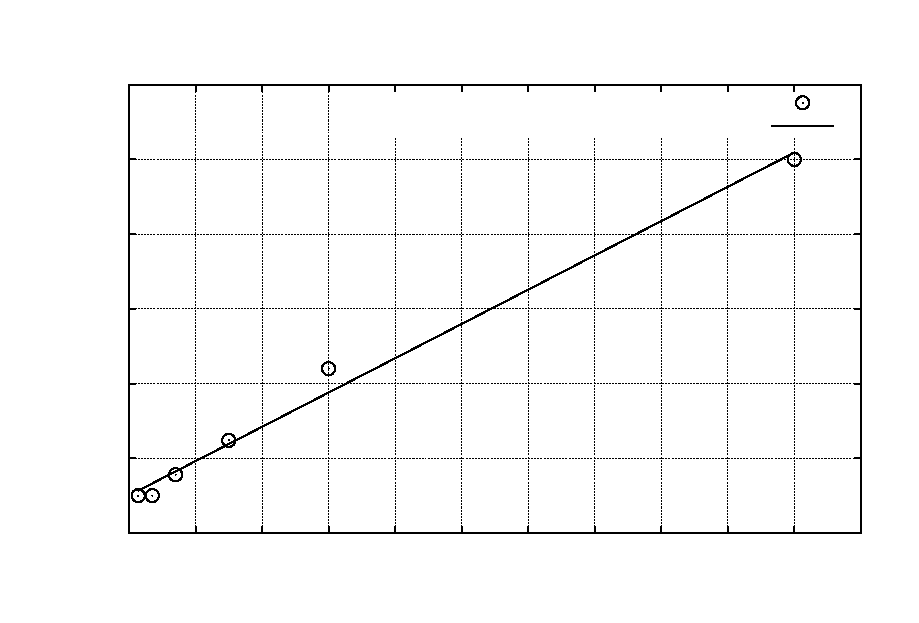
\includegraphics{fig1}}%
    \gplfronttext
  \end{picture}%
\endgroup

	\caption{%
		Runtime for the Hadoop-based pipeline on the 56-core Hadoop cluster with
		increasing input dataset size. Each test dataset (labelled with Roman
		numerals) was used. The image clearly highlights the linear scaling
		characteristics of the Hadoop-based approach.
		}
	\label{fig:fig1}
\end{figure}


\begin{figure}[!ht]
	% GNUPLOT: LaTeX picture with Postscript
\begingroup
  \makeatletter
  \providecommand\color[2][]{%
    \GenericError{(gnuplot) \space\space\space\@spaces}{%
      Package color not loaded in conjunction with
      terminal option `colourtext'%
    }{See the gnuplot documentation for explanation.%
    }{Either use 'blacktext' in gnuplot or load the package
      color.sty in LaTeX.}%
    \renewcommand\color[2][]{}%
  }%
  \providecommand\includegraphics[2][]{%
    \GenericError{(gnuplot) \space\space\space\@spaces}{%
      Package graphicx or graphics not loaded%
    }{See the gnuplot documentation for explanation.%
    }{The gnuplot epslatex terminal needs graphicx.sty or graphics.sty.}%
    \renewcommand\includegraphics[2][]{}%
  }%
  \providecommand\rotatebox[2]{#2}%
  \@ifundefined{ifGPcolor}{%
    \newif\ifGPcolor
    \GPcolorfalse
  }{}%
  \@ifundefined{ifGPblacktext}{%
    \newif\ifGPblacktext
    \GPblacktexttrue
  }{}%
  % define a \g@addto@macro without @ in the name:
  \let\gplgaddtomacro\g@addto@macro
  % define empty templates for all commands taking text:
  \gdef\gplbacktext{}%
  \gdef\gplfronttext{}%
  \makeatother
  \ifGPblacktext
    % no textcolor at all
    \def\colorrgb#1{}%
    \def\colorgray#1{}%
  \else
    % gray or color?
    \ifGPcolor
      \def\colorrgb#1{\color[rgb]{#1}}%
      \def\colorgray#1{\color[gray]{#1}}%
      \expandafter\def\csname LTw\endcsname{\color{white}}%
      \expandafter\def\csname LTb\endcsname{\color{black}}%
      \expandafter\def\csname LTa\endcsname{\color{black}}%
      \expandafter\def\csname LT0\endcsname{\color[rgb]{1,0,0}}%
      \expandafter\def\csname LT1\endcsname{\color[rgb]{0,1,0}}%
      \expandafter\def\csname LT2\endcsname{\color[rgb]{0,0,1}}%
      \expandafter\def\csname LT3\endcsname{\color[rgb]{1,0,1}}%
      \expandafter\def\csname LT4\endcsname{\color[rgb]{0,1,1}}%
      \expandafter\def\csname LT5\endcsname{\color[rgb]{1,1,0}}%
      \expandafter\def\csname LT6\endcsname{\color[rgb]{0,0,0}}%
      \expandafter\def\csname LT7\endcsname{\color[rgb]{1,0.3,0}}%
      \expandafter\def\csname LT8\endcsname{\color[rgb]{0.5,0.5,0.5}}%
    \else
      % gray
      \def\colorrgb#1{\color{black}}%
      \def\colorgray#1{\color[gray]{#1}}%
      \expandafter\def\csname LTw\endcsname{\color{white}}%
      \expandafter\def\csname LTb\endcsname{\color{black}}%
      \expandafter\def\csname LTa\endcsname{\color{black}}%
      \expandafter\def\csname LT0\endcsname{\color{black}}%
      \expandafter\def\csname LT1\endcsname{\color{black}}%
      \expandafter\def\csname LT2\endcsname{\color{black}}%
      \expandafter\def\csname LT3\endcsname{\color{black}}%
      \expandafter\def\csname LT4\endcsname{\color{black}}%
      \expandafter\def\csname LT5\endcsname{\color{black}}%
      \expandafter\def\csname LT6\endcsname{\color{black}}%
      \expandafter\def\csname LT7\endcsname{\color{black}}%
      \expandafter\def\csname LT8\endcsname{\color{black}}%
    \fi
  \fi
  \setlength{\unitlength}{0.0500bp}%
  \begin{picture}(8502.00,5668.00)%
    \gplgaddtomacro\gplbacktext{%
      \csname LTb\endcsname%
      \put(946,704){\makebox(0,0)[r]{\strut{} 1.1}}%
      \csname LTb\endcsname%
      \put(946,1319){\makebox(0,0)[r]{\strut{} 1.2}}%
      \csname LTb\endcsname%
      \put(946,1933){\makebox(0,0)[r]{\strut{} 1.3}}%
      \csname LTb\endcsname%
      \put(946,2548){\makebox(0,0)[r]{\strut{} 1.4}}%
      \csname LTb\endcsname%
      \put(946,3163){\makebox(0,0)[r]{\strut{} 1.5}}%
      \csname LTb\endcsname%
      \put(946,3778){\makebox(0,0)[r]{\strut{} 1.6}}%
      \csname LTb\endcsname%
      \put(946,4392){\makebox(0,0)[r]{\strut{} 1.7}}%
      \csname LTb\endcsname%
      \put(946,5007){\makebox(0,0)[r]{\strut{} 1.8}}%
      \csname LTb\endcsname%
      \put(1078,484){\makebox(0,0){\strut{} 0}}%
      \csname LTb\endcsname%
      \put(1956,484){\makebox(0,0){\strut{} 0.02}}%
      \csname LTb\endcsname%
      \put(2835,484){\makebox(0,0){\strut{} 0.04}}%
      \csname LTb\endcsname%
      \put(3713,484){\makebox(0,0){\strut{} 0.06}}%
      \csname LTb\endcsname%
      \put(4592,484){\makebox(0,0){\strut{} 0.08}}%
      \csname LTb\endcsname%
      \put(5470,484){\makebox(0,0){\strut{} 0.1}}%
      \csname LTb\endcsname%
      \put(6348,484){\makebox(0,0){\strut{} 0.12}}%
      \csname LTb\endcsname%
      \put(7227,484){\makebox(0,0){\strut{} 0.14}}%
      \csname LTb\endcsname%
      \put(8105,484){\makebox(0,0){\strut{} 0.16}}%
      \put(176,2855){\rotatebox{-270}{\makebox(0,0){\strut{}ratio of $F_{Hadoop}/F_{HPC}$}}}%
      \put(4591,154){\makebox(0,0){\strut{}reciprocal dataset size, 1/Gbases}}%
      \put(4591,5337){\makebox(0,0){\strut{}Figure 2}}%
    }%
    \gplgaddtomacro\gplfronttext{%
      \csname LTb\endcsname%
      \put(7578,4423){\makebox(0,0){\strut{}datasetI}}%
      \put(4240,2394){\makebox(0,0){\strut{}datasetII}}%
      \put(2747,1595){\makebox(0,0){\strut{}datasetIII}}%
      \put(1737,919){\makebox(0,0){\strut{}datasetIV}}%
      \csname LTb\endcsname%
      \put(1310,4834){\makebox(0,0)[l]{\strut{}least-squares fit to $y=aX+b$ for the data with  $b=1.13$}}%
    }%
    \gplbacktext
    \put(0,0){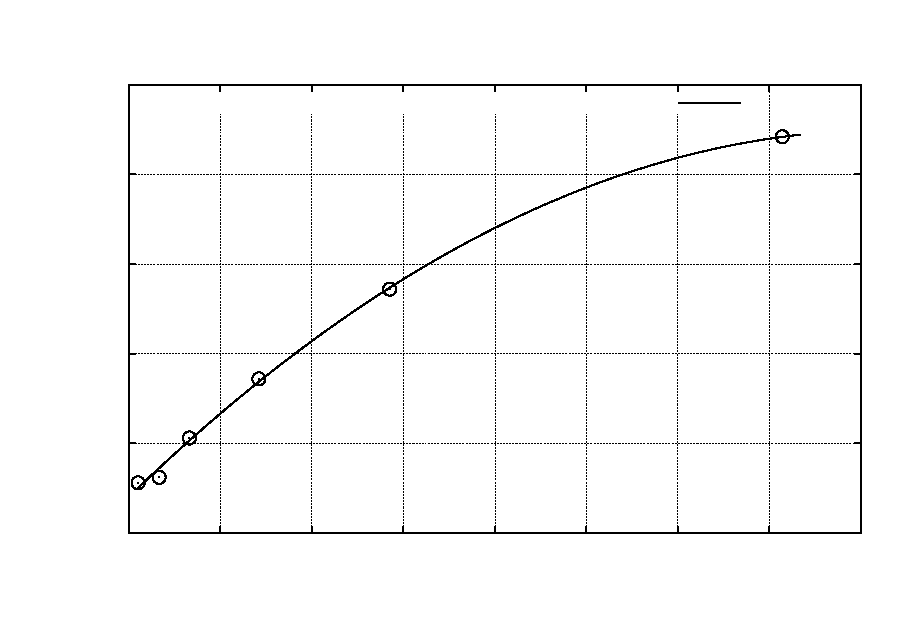
\includegraphics{fig2}}%
    \gplfronttext
  \end{picture}%
\endgroup

	\caption{%
	The ratio of the~$F_{Hadoop}/F_{HPC}$ as a function of a reciprocal
	dataset size in Gbases. The pipelines were run on a 56-core Hadoop cluster and
	a 16-core HPC node, respectively.
	The points are fit to a quadratic least-squares curve, which makes it possible
	to predict {\it infinite} dataset size. Datasets are labeled with Roman
	numerals.
	}
	\label{fig:fig2}
\end{figure}


\begin{figure}[!ht]
	\small
	% GNUPLOT: LaTeX picture with Postscript
\begingroup
  \makeatletter
  \providecommand\color[2][]{%
    \GenericError{(gnuplot) \space\space\space\@spaces}{%
      Package color not loaded in conjunction with
      terminal option `colourtext'%
    }{See the gnuplot documentation for explanation.%
    }{Either use 'blacktext' in gnuplot or load the package
      color.sty in LaTeX.}%
    \renewcommand\color[2][]{}%
  }%
  \providecommand\includegraphics[2][]{%
    \GenericError{(gnuplot) \space\space\space\@spaces}{%
      Package graphicx or graphics not loaded%
    }{See the gnuplot documentation for explanation.%
    }{The gnuplot epslatex terminal needs graphicx.sty or graphics.sty.}%
    \renewcommand\includegraphics[2][]{}%
  }%
  \providecommand\rotatebox[2]{#2}%
  \@ifundefined{ifGPcolor}{%
    \newif\ifGPcolor
    \GPcolorfalse
  }{}%
  \@ifundefined{ifGPblacktext}{%
    \newif\ifGPblacktext
    \GPblacktexttrue
  }{}%
  % define a \g@addto@macro without @ in the name:
  \let\gplgaddtomacro\g@addto@macro
  % define empty templates for all commands taking text:
  \gdef\gplbacktext{}%
  \gdef\gplfronttext{}%
  \makeatother
  \ifGPblacktext
    % no textcolor at all
    \def\colorrgb#1{}%
    \def\colorgray#1{}%
  \else
    % gray or color?
    \ifGPcolor
      \def\colorrgb#1{\color[rgb]{#1}}%
      \def\colorgray#1{\color[gray]{#1}}%
      \expandafter\def\csname LTw\endcsname{\color{white}}%
      \expandafter\def\csname LTb\endcsname{\color{black}}%
      \expandafter\def\csname LTa\endcsname{\color{black}}%
      \expandafter\def\csname LT0\endcsname{\color[rgb]{1,0,0}}%
      \expandafter\def\csname LT1\endcsname{\color[rgb]{0,1,0}}%
      \expandafter\def\csname LT2\endcsname{\color[rgb]{0,0,1}}%
      \expandafter\def\csname LT3\endcsname{\color[rgb]{1,0,1}}%
      \expandafter\def\csname LT4\endcsname{\color[rgb]{0,1,1}}%
      \expandafter\def\csname LT5\endcsname{\color[rgb]{1,1,0}}%
      \expandafter\def\csname LT6\endcsname{\color[rgb]{0,0,0}}%
      \expandafter\def\csname LT7\endcsname{\color[rgb]{1,0.3,0}}%
      \expandafter\def\csname LT8\endcsname{\color[rgb]{0.5,0.5,0.5}}%
    \else
      % gray
      \def\colorrgb#1{\color{black}}%
      \def\colorgray#1{\color[gray]{#1}}%
      \expandafter\def\csname LTw\endcsname{\color{white}}%
      \expandafter\def\csname LTb\endcsname{\color{black}}%
      \expandafter\def\csname LTa\endcsname{\color{black}}%
      \expandafter\def\csname LT0\endcsname{\color{black}}%
      \expandafter\def\csname LT1\endcsname{\color{black}}%
      \expandafter\def\csname LT2\endcsname{\color{black}}%
      \expandafter\def\csname LT3\endcsname{\color{black}}%
      \expandafter\def\csname LT4\endcsname{\color{black}}%
      \expandafter\def\csname LT5\endcsname{\color{black}}%
      \expandafter\def\csname LT6\endcsname{\color{black}}%
      \expandafter\def\csname LT7\endcsname{\color{black}}%
      \expandafter\def\csname LT8\endcsname{\color{black}}%
    \fi
  \fi
  \setlength{\unitlength}{0.0500bp}%
  \begin{picture}(8502.00,5668.00)%
    \gplgaddtomacro\gplbacktext{%
      \csname LTb\endcsname%
      \put(946,704){\makebox(0,0)[r]{\strut{} 0}}%
      \put(946,1242){\makebox(0,0)[r]{\strut{} 0.5}}%
      \put(946,1780){\makebox(0,0)[r]{\strut{} 1}}%
      \put(946,2318){\makebox(0,0)[r]{\strut{} 1.5}}%
      \put(946,2856){\makebox(0,0)[r]{\strut{} 2}}%
      \put(946,3393){\makebox(0,0)[r]{\strut{} 2.5}}%
      \put(946,3931){\makebox(0,0)[r]{\strut{} 3}}%
      \put(946,4469){\makebox(0,0)[r]{\strut{} 3.5}}%
      \put(946,5007){\makebox(0,0)[r]{\strut{} 4}}%
      \put(1078,484){\makebox(0,0){\strut{} 0}}%
      \put(2483,484){\makebox(0,0){\strut{} 0.05}}%
      \put(3889,484){\makebox(0,0){\strut{} 0.1}}%
      \put(5294,484){\makebox(0,0){\strut{} 0.15}}%
      \put(6700,484){\makebox(0,0){\strut{} 0.2}}%
      \put(8105,484){\makebox(0,0){\strut{} 0.25}}%
      \put(176,2855){\rotatebox{-270}{\makebox(0,0){\strut{}$T_{mapping}/T_{comm}$}}}%
      \put(4591,154){\makebox(0,0){\strut{}reciprocal number of nodes, $1/N$}}%
      \put(4591,5337){\makebox(0,0){\strut{}Ratios of the  short reads mapping time per node to the communication  time}}%
    }%
    \gplgaddtomacro\gplfronttext{%
      \csname LTb\endcsname%
      \put(7118,1977){\makebox(0,0)[r]{\strut{}HPC SLURM}}%
      \csname LTb\endcsname%
      \put(7118,1757){\makebox(0,0)[r]{\strut{}Hadoop}}%
      \csname LTb\endcsname%
      \put(7118,1537){\makebox(0,0)[r]{\strut{}HPC random}}%
      \csname LTb\endcsname%
      \put(7118,1317){\makebox(0,0)[r]{\strut{}linear fit for Hadoop }}%
      \csname LTb\endcsname%
      \put(7118,1097){\makebox(0,0)[r]{\strut{}linear fit for HPC SLURM}}%
      \csname LTb\endcsname%
      \put(7118,877){\makebox(0,0)[r]{\strut{}linear fit for HPC random}}%
    }%
    \gplbacktext
    \put(0,0){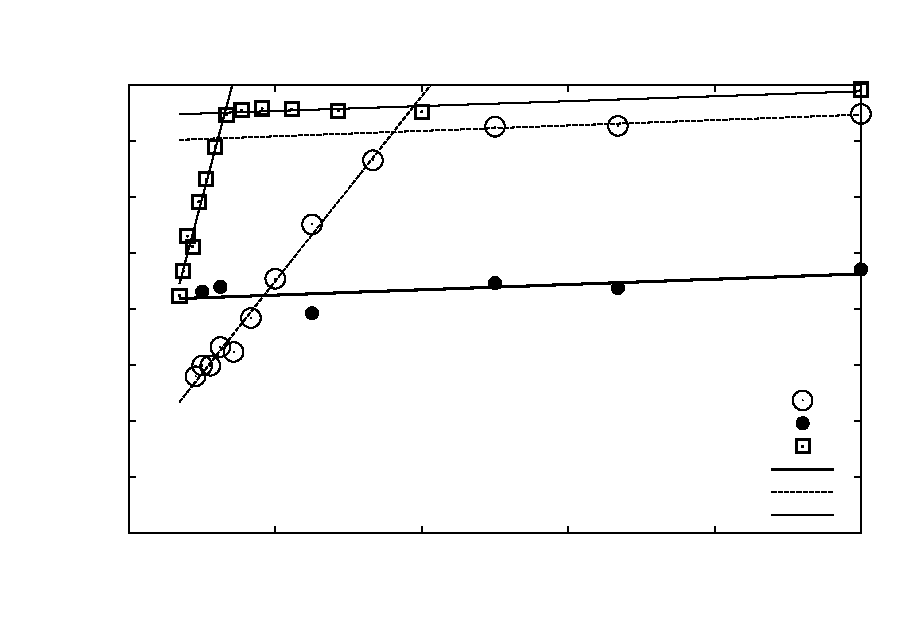
\includegraphics{fig3}}%
    \gplfronttext
  \end{picture}%
\endgroup

	\normalsize
\caption{%
	Ratios of alignment time~$T_{alignment}$ to communication costs~$T_{comm}$ for
	the HPC and Hadoop clusters as a function of reciprocal number of nodes~$1/N$.
	All runs used Dataset~IV as input. Two HPC scenarios are shown as ``HPC
	SLURM'' and ``HPC random'', which correspond to standard SLURM behavior and a
	modified one that allocates nodes from random racks.  Linear fit to $ax+b$ was
	done with the least-squares method.  The estimated coefficients for the
	Hadoop-based approach are $(a,b)\approx(0.95,2.07)$.  One can see two defined
	linear regions for the HPC approach with very different tangents for linear
	and non-linear scalings correspondingly.  For  the ``HPC SLURM'' $(a,b)\approx
	(0.96, 3.49)$ and $(a,b)\approx (32.99, 0.60)$, and for  the ``HPC random''
	$(a,b)\approx (0.88, 3.72)$ and $(a,b)\approx (98.24, 0.53)$.  The constant
	term for HPC goes below unity -- i.e.\ for a large number of nodes more time
	will be spent on communication than the actual alignment. 
	}

%The first one resembles to that of Hadoop, and corresponds to the case then the communication in the cluster is not a bottleneck. 
%The second one shows the regime corresponding to the case of saturation of the network, resulting in traffic jams: data distibution time~$T_{comm}$ stops to scale 
%linearly to the reciprocal cluster size, and becomes more of less a constant, while the alignment time continues to satisfy~$T_{alignment}\propto 1/N$.
	\label{fig:fig3}
\end{figure}

\begin{figure}[!ht]
 	\begin{subfigure}[b]{0.4\textwidth}
        	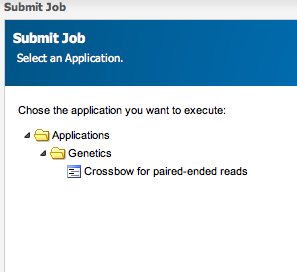
\includegraphics[width=\textwidth]{a.png}
		\subcaption{}
	\end{subfigure}
	\hspace{0.5cm}
	\begin{subfigure}[b]{0.6\textwidth}
	        	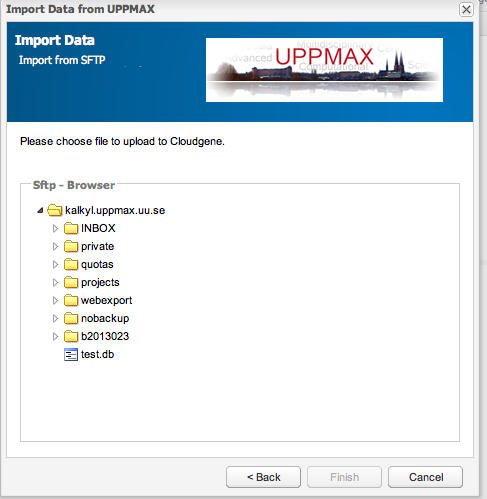
\includegraphics[width=\textwidth]{c.png}
		\subcaption{}
	\end{subfigure}
%	\begin{subfigure}[b]{0.6\textwidth}
%		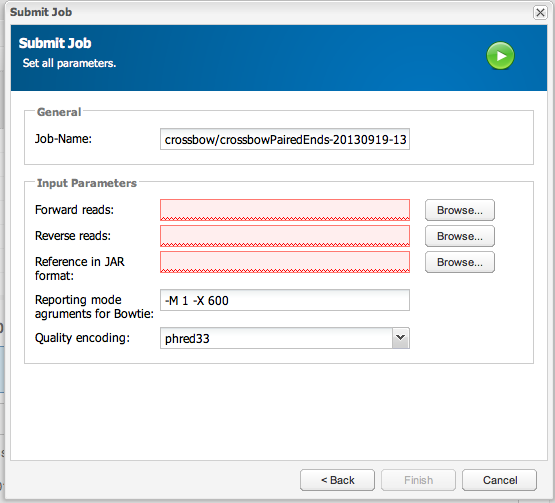
\includegraphics[width=\textwidth]{b.png}
%		\subcaption{Cloudgene: specifying job parameters}
%	\end{subfigure}
	\caption{%
	An example of a job setup view with the graphical Hadoop front-end Cloudgene,
	providing a smooth user experience even for novice users. \textbf{a)} Pipeline
	selection -- in our case containing the Crossbow pipeline. \textbf{b)} The
	UPPMAX-adapted functionality to browsing and import data from the user's home
	folder in the shared file system.
	}
	\label{fig:fig4}
\end{figure}



%%%%%%%%%%%
% Tables
%%%%%%%%%%%
\section*{Tables}

\begin{table}[!ht]
\small
\footnotesize
\caption{Datasets used in the comparison. }
\begin{center}
\begin{tabular}{|l|l|l|}
Dataset &	Organism &	Size in Gbases\\
\hline
 I		&	{\it A.thaliana}	&	1.4	\\
 II	&	{\it A.thaliana}	&	7.0\\
 III	&	{\it A.thaliana}	&	30.0	\\
 IV	&{\it A.thaliana}, the artificial dataset created using Samtools package	&	100.0	\\
 V	&	{\it H.sapiens}, two individuals (GM12750 and GM12004), sample SRR499924		&	250.0\\

\end{tabular}
\end{center}
\label{table:datasets}
\normalsize
\end{table}%


\begin{table}[!ht]
\small
\caption{%
	Time (in minutes) employed to preprocess Datasets II, III, and IV by
	Crossbow's native read preprocessor and our MR preprocessor on a 56-core Hadoop
	cluster, and by the custom multi-core Bash script on a single 16-core HPC node.
	}

\begin{center}
\begin{tabular}{l|c|c|c}
Dataset			&		II (7 Gbases )	& III (30 Gbases)	& IV (100 Gbases)\\
\hline
Crossbow native			&		$60.6\pm0.7$	& $299.0\pm2.3$	&	$673.0\pm1.0$	\\
Hadoop, this work			&		$7.0\pm0.0$	&	$20.7\pm0.4$&		$52.4\pm0.1$\\
Bash, this work			& 		$7.4\pm0.0$	&	$31.1\pm0.1$	&	$114.5\pm0.3$	\\
\end{tabular}
\end{center}
\label{table:preprocess}
\normalsize
\end{table}%




\begin{table}[!ht]
\small

\caption{%
	Time (in minutes) for processing different dataset sizes on the HPC and
	Hadoop deployments with their respective pipelines. Datasets are labelled by
	Roman numerals, (``f.r.'' stands for ``forward reads''). The large variance
	for the HPC deployment is due to Samtools BAM sorting, which is I/O and memory
	intensive; the data spillage to the file system makes it very susceptible to
	the load of the entire shared HPC cluster.
	}

\begin{center}
\begin{tabular}{l|c|c|c|c|c|c|c}

Data, Gbases		&	1.4	&	3.5		&	7.0		&	15.0		&	30.0		&	100.0	&	250 	\\
				&	(I)	&	(II, f.r.)	&	(II)		&	(III, f.r.)	&	(III)		&	(IV)		&	(V)\\
\hline
Hadoop, 56 cores		&	$18\pm0	$	&	$18\pm0	$	&	$29\pm0$	&	$47\pm0	$	&	$89\pm0$	&	$238\pm1$		&	$1164\pm14$\\
HPC, 16 cores	&	$17\pm1$	&	$22\pm6$	&	$43\pm3$	&	$81\pm9$	&	$172\pm15$		&	$467\pm60$	& $>48$ hours\\

\end{tabular}
\end{center}
\label{table:pipleline-timings}
\normalsize
\end{table}%




\begin{table}[!ht]
\small
\caption{Timings for Dataset I processed on different number of cores of a HPC node.}
\begin{center}
\begin{tabular}{c|c|c|c|ccc}
$N$ cores	&\multicolumn{3}{c|}{timing, minutes}&\multicolumn{3}{c}{speed-ups} \\
\hline
	& alignment 	&	SNP calling	&	total  &total & alignment& SNP call\\
\hline
1	&	22.75	$\pm$1.24&	26.1$\pm$0.7	&	48.9	&	 1.00	&	1.00	&	1.00\\
2	&	11.00$\pm$0.05	&	16.9$\pm$1.3	&	27.9	&	 0.88	&	1.03	&	0.77\\
4	&	5.91$\pm$0.04	&	11.7$\pm$0.5	&	17.6	&	 0.69	&	0.96	&	0.56\\
6	&	4.24$\pm$0.04	&	8.6$\pm$0.8	&	12.8	&	 0.64	&	0.89	&	0.51\\
8	&	3.44$\pm$0.03	&	8.6$\pm$0.9	&	12.1	&	 0.51	&	0.83	&	0.38\\
10	&	2.91$\pm$0.01	&	7.7$\pm$0.5	&	10.6	&	 0.46	&	0.78	&	0.34\\
12	&	2.64$\pm$0.04	&	7.5$\pm$0.5	&	10.1	&	 0.40	&	0.72	&	0.29\\
14	&	2.57$\pm$0.03	&	7.5$\pm$0.6	&	10.1	&	 0.35	&	0.63	&	0.25\\
16	&	2.88$\pm$0.06	&	7.4$\pm$0.4	&	10.2	&	 0.30	&	0.49	&	0.22\\
\end{tabular}
\end{center}
\label{table:timings-hpc}
\normalsize
\end{table}


 \begin{table}[hbtp]
\small

\caption{%
	Time (in minutes) required by Samtools to sort
	Dataset IV (BAM file containing 58 Gbases). The measurements are done on a single HPC
	node with $p=16$ cores. Averaging is done over 5 independent simulations. The
	amount of available RAM reported is for all 16 cores.
}
\begin{center}
\begin{tabular}{|l|c|c|c|c|c|c|c|}
RAM, GB		&	8			&		16			&			32		& 		64				\\
timing, minutes	&	$208\pm50$	&	$172\pm13$		&	$136\pm12$		& 	$87\pm11$			\\
\end{tabular}
\end{center}
\label{table:samtools-sort}
\normalsize
\end{table}%






\begin{table}[!ht]
\caption{Timings  for alignment and the ratio~$T_{alignment}/T_{comm}$ for HPC and Hadoop clusters for Dataset IV.
For the ``HPC random'' approach, data chunks have to be copied to the local scratch disks first and the alignments (SAM files) copied back while Hadoop keeps all the data inside HDFS and hence does not need data staging. Hadoop however needs to preprocess reads before the actual alignment stage in order to be able to operate in MR manner resulting in what we term ``communication costs''. Note that each HPC node has 16 cores, while each Hadoop node has 7 (one core is dedicated to run the virtual machine).}
\begin{center}
\begin{tabular}{c|c|c|c|c|c}
 \multicolumn{3}{c|}{Hadoop} & \multicolumn{3}{c}{HPC random} \\
 \hline		


Number of nodes	&Alignment time,	&$\frac{T_{alignment}}{T_{comm}}$	&Number of nodes	&Alignment time,	&$\frac{T_{alignment}}{T_{comm}}$\\
(cores)					&minutes		&							&(cores)			&minutes&\\
\hline
4(28)	&293.5	&2.33	&4(64)	&74.4	&3.89\\
6(42)	&189.8	&2.19	&10(160)	&32.4	&3.76\\
8(56)	&136.0	&2.23	&14(224)	&22.7	&3.77\\
16(112)	&70.3	&1.96	&18(288)	&17.9	&3.78\\
32(224)	&39.3	&2.20	&22(352)	&14.5	&3.79\\
40(280)	&32.5	&2.15	&26(416)	&12.3	&3.77\\
			&&&30(480)	&10.7	&3.73\\
			&&&34(544)	&9.5	&3.45\\
			&&&38(608)	&8.5	&3.16\\
			&&&42(672)	&7.6	&2.96\\
			&&&46(736)	&7.0	&2.55\\
			&&&50(800)	&6.4	&2.65\\
			&&&54(864)	&5.9	&2.34\\
			&&&58(928)	&5.5	&2.12\\

\end{tabular}
\end{center}
\label{table:timings-algn}
\end{table}%

\end{document}

